\documentclass[class=book, crop=false, oneside, 12pt]{standalone}
\usepackage{standalone}
\usepackage{../../style}
\graphicspath{{./assets/images/}}

\begin{document}

\chapter{provvisori(ssim)o}

\section{Analisi lessicale}
\subsection{Introduzione}
Dopo i precedenti due capitoli, nei quali abbiamo introdotto e approfondito un buono numero di concetti, algoritmi e modelli necessari alla comprensione di come l'impostazione teorica dei linguaggi formali sia fondamentale nella progettazione dei compilatori, andiamo a tuffarci in quella che è la prima fase di compilazione: l'analisi lessicale.


Ricordiamo che questa è la fase in cui vogliamo identificare quali parti del sorgente che abbiamo scritto corrispondono alle keyword, quali agli identificatori,alle costanti, e via di questo passo; per essere più formali, questi elementi che vogliamo riconoscere portano il nome di \emph{lessemi}, e trasformare quindi il sorgente in un flusso di tokens, i quali costituiscono i terminali della grammatica che genera il nostro linguaggio di programmazione.

La grammaticafi un linguaggio ci dirà quali sono le forme che un'espressione deve avere per essere considerata ben formata rispetto a quel linguaggio. Ad esempio, una grammatica ci può dire che la seguente forma denota un'espressione valida:\\
% begin minted
Identificatore      simbolo di assegnamento    numero\\
% end minted
e che quindi espressioni ome la seguente sono grammaticali e ben formate secondo il linguaggio.\\
% begin minted
pippo = 2\\
% end minted8
Il mestiere dell'analizzatore lessicale è proprio quello di ricevere in input un \texttt{pippo} qualsiasi (che è un token) e, in output, determinare che è un \emph{identificatore}, ossia la categoria più astratta (lessema) di cui \texttt{pippo} è istanza.

% L’analizzatore lessicale lavora in tandem (pipeline) con l’analizzatore sintattico per non si sa bene come o perché
\subsection{Esempio: la grammatica di C99}
Andiamo a vedere da vicino la grammatica di un reale linguaggio, anzi, del linguaggio preferito di tutti noi, ossia il C (nella versione \(99\), scritta per il parser \emph{Bison}); il lettore interessato ad approfondire può trovare lo stesso file cliccando \href{./assets/files/c99.y}{qui} (fonte: \url{http://www.quut.com/c/ANSI-C-grammar-y-1999.html}).
\begin{figure}[H]
    \centering
    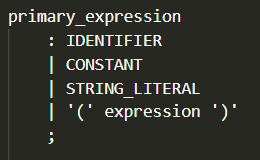
\includegraphics[width=.4\textwidth,keepaspectratio]{c99-ex1}
    \caption{}
    % \label{dfa-b_odd-and-a_even}
\end{figure}
Notiamo subito alcune differenze rispetto alla notazione che abbiamo impiegato finora: 
\begin{itemize}
    \item la freccia ( \(\to\) ) è rappresentata da un altro simbolo, i due punti ( \(:\) );
    \item il pipe ( \(\mid\) ), invece, possiede il medesimo significato;
    \item i terminali possono essere indicati precisamente con '';
    \item inoltre, la convenzione rispetto alla capitalizzazione è invertita: qui osserviamo che gli elementi in maiuscolo sono i terminali, mentre invece quelli in minuscolo rappresentano non terminali; ad esempio, in figura sopra possiamo notare che il non-letterale \texttt{primary\_expression} ha una produzione per cui può risultare o in una serie di letterali (\texttt{IDENTIFIER}, \texttt{CONSTANT}), oppure in una forma \texttt{'(' expression ')'}, dove \texttt{expression} è un altro non letterale, che a sua volta avrà altre produzioni.
\end{itemize}

Questo file, inoltre, è pensato per essere utilizzato in tandem con un analizzatore sintattico; per questo motivo, nell'intestazione dello stesso possiamo trovare le dichiarazione di quelli che sono i token (vale a dire, lo ripetiamo, i terminali della grammatica descritta). Saranno espressi in questa forma:
\begin{figure}[H]
    \centering
    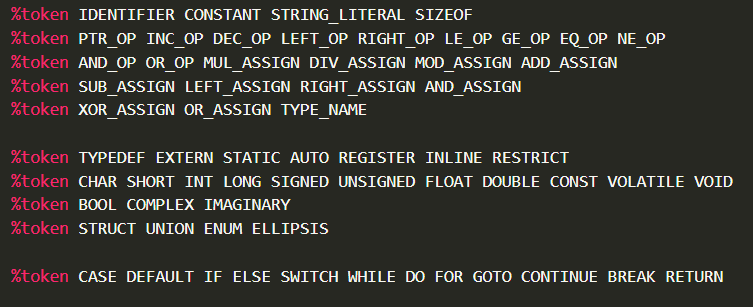
\includegraphics[width=.7\textwidth,keepaspectratio]{c99-ex2}
    \caption{}
    % \label{dfa-b_odd-and-a_even}
\end{figure}

Un'altra cosa che possiamo osservare è la dichiarazione di quello che è lo starting symbol della grammatica:\\
% begin minted
\% start translation\_unit\\
% end minted
Questa dichiarazione in realtà potrebbe non essere presente su alcuni file contenenti grammatiche, dal momento che, in sua assenza, non otteniamo degli errori, bensì viene preso il non-letterale della prima produzione listata a seguito come starting symbol.

Il ruolo dell’analizzatore lessicale è quindi analizzare il sorgente e decidere, di volta in volta, quale derivazione può essere applicata a ciascuna delle righe del sorgente analizzato. Una volta completato l'albero di derivazione e quindi arrivato presso un terminale (ad esempio \texttt{IDENTIFIER}), l'analizzatore lessicale andrà anche ad associargli un valore, dal momento che è necessario distinguere quell'\texttt{IDENTIFIER} da un altro; questo è necessario, perché nel programma potremmo tranquillamente avere due \texttt{IDENTIFIER} di diverso tipo, o in ogni caso potremmo comunque voler conservare delle informazioni aggiuntive di qualche tipo (nome, scope e altro ancora). Tutte queste informazioni vengono conservate in una \emph{symbol table}.

Infine, le ultime rihe del file contengono informazioni utili al particolare analizzatore sintattico utilizzato; avremo modo di parlarne nel dettaglio in futuro.

\subsection{Classi di tokens}
Si potrebbe a ragione considerare superfluo specificare che ogni diversa grammatica (e quindi ogni linguaggio) presenta diverse categorie di tokens; banalmente, il lettore è probabilmente ben cosciente che linguaggi diversi possiedono generalmente keyword diverse. Ad ogni modo, a seguito presentiamo alcune tra le scelte più ricorrenti:
\begin{itemize}
    \item un token per ogni keyword, quindi un token per ogni nome di base già presente nel linguaggio (\texttt{if}, \texttt{while}, \texttt{for} e via dicendo;
    \item un token per ogni operatore (o anche per classe di operatori), quindi in C ne avremo uno per \texttt{+} ma anche uno dedicato per \texttt{++}; 
    \item un unico token per gli identificatori, valido per tutti quanti;
    \item un token per ogni simbolo di punteggiatura. 
\end{itemize}

\subsection{Il lavoro dell'analizzatore lessicale}
L'obiettivo dell'analalizzatore lessicale è quindi riconoscere i cosiddetti \emph{lessemi}, ossia quelle parti del programma che corrispondono ai token, e ritornarli. Ciascuno di questi, di solito, vengono ritornati sotto forma di coppia \texttt{<token-name>: <token-value>}, dove:
\begin{itemize}
    \item \texttt{<token-name>} è il nome scelto per denotare quel preciso token; seguendo l'esempio della grammatica precedente, \texttt{IDENTIFIER} è un \texttt{<token-name>};
    \item \texttt{<token-value>} è tipicamente un puntatore a una entry della symbol table, in cui si va a salvare tutte le informazioni relative a quel preciso token di tipo\footnote{In questo caso la parola "tipo" è chiaramente impropria, ma è molto utile per rendere la natura astratta di classe di token.} \texttt{<token-name>}.
\end{itemize}

\subsection{Lessemi e espressioni regolari}
Andiamo quindi a capire in che modo la teoria studiata nei due capitoli precedenti entra prepotentemente nell'analisi lessicale.

I lessemi sono estremamente facili da descrivere utilizzando le espressioni regolari: ad esempio, in un linguaggio che prevede un lessema identificatore, il quale è costituito di qualsiasi combinazione di lettere maiuscole e minuscole, quest'ultimo può essere facilmente denotato da un'espressione regolare del tipo:
\begin{equation*}
    (a \mid b \mid \ldots \mid z \mid A \mid B \mid \ldots \mid Z)^*
\end{equation*}
Questo è molto interessante: se è vero che i lessemi sono perfettamente descrivibili con dei linguaggi regolari, allora vuol dire che possiamo utilizzare quelli in sede di analisi lessicale, senza dover tirare in ballo i più potenti ma decisamente più complessi linguaggi liberi.

Quindi questi lessemi, essendo descritti da delle espressioni regolari, possono anche essere riconosciuti agevolmente da una macchina a stati, come ad esempio quella in figura sotto, che descrive la classe \texttt{relop} di token per gli operatori relazionali.
\begin{figure}[H]
    \centering
    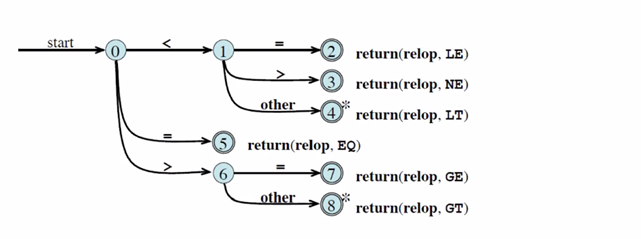
\includegraphics[width=\textwidth,keepaspectratio]{lec-14-1}
    \caption{}
    % \label{dfa-b_odd-and-a_even}
\end{figure}
È molto semplice intuire graficamente che ciascun percorso che termini in uno stato finale ritorna un token, sotto forma di coppia, in cui il \texttt{token-name} è appunto quello della classe \texttt{relop}, mentre il \texttt{token-value} indica qual è l'elemento della classe da ritornare.

\paragraph{Retract}
Possiamo notare che i due stati finali il cui arco entrante è marcato come \(other\) hanno anche un asterisco: questo indica che, quando consumo quella transizione, devo ricordarmi di tornare indietro di una parola, perché quest'ultima parola \(other\) (cioè che non fa parti di alcun elemento appartenente alla classe \texttt{relop}) potrebbe essere un elemento di un token successivo, e se non compiano quanto detto sopra rischieremmo di saltarla nell'analisi e ottenere un flusso di token incorretto. Questa operazione è detta \(retract\).

L'operazione di retract è unodei tanti elementi legati alla gestione dell'input e del buffer che ci fanno pensare che la macchina a stati è un modello molto vicino al più noto, per noi, automa a stati finiti, ma quanto è profondo questo legame?

\subsection{Pattern matching basato su NFA}
Immaginiamo di avere delle espressioni regolari che denotano il linguaggio dei lessemi che siamo interessati a riconoscere. Si pensi ad esempio all'espressione regolare che denota il lessema \texttt{IDENTIFIER}, ossia l'espressione regolare che denota tutte le possibili combinazioni di lettere maiuscole e minuscole (con le dovute peculiarità di ciascun linguaggio); oppure, si pensi a un'espressione regolare che denoti il lessema degli operatori relazionali, o ancora un'altra che denoti la scrittura dei floating numbers. In sostanza, per ciascuna categoria sintattica abbiamo un'espressione regolare che la denota.

Sappiamo anche che, avendo delle espressioni regolari, per ciascuna di queste possiamo costruire degli NFA che riconoscono il linguaggio denotato dall'espressione considerata; possiamo a questo punto immaginare di far collidere questi NFA inserendo uno stato iniziale extra e collegandolo a ciascun NFA tramite una \(\varepsilon\)-transizione, come mostrato in figura sotto.
\begin{figure}[H]
    \centering
    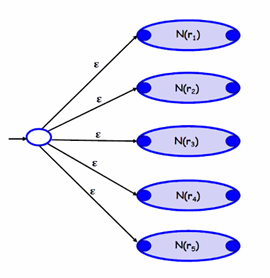
\includegraphics[width=.4\textwidth,keepaspectratio]{lec-14-2}
    \caption{}
    % \label{dfa-b_odd-and-a_even}
\end{figure}
Una struttura di questo tipo può riconoscere i linguaggi denotati da tutte le espressioni regolari per cui abbiamo costruito degli NFA. 

Adesso dobbiamo pensare come ottimizzare l'uso di una struttura simile per l'analisi lessicale. Potremmo trovarci infatti a gestire problemi di diversa natura, in particolare relativi all'input buffering: ad esempio, come posso fare a sapere se i due caratteri \texttt{i} e \texttt{f} che ho appena letto stanno a indicare la keyword \texttt{if} e non un ipotetico identificatore \texttt{iffoff}? Detto in maniera informale, come decido quando fermarmi, quando tornare indietro, quando e se ho letto più di quanto mi serviva?

Il procedimento che seguiamo è il seguente:
\begin{enumerate}
    \item innanzitutto simuliamo l'NFA creato come sopra descritto;
    \item ci sono delle azioni associate agli stati finali;
    \item nel caso di ambiguità, ossia di situazioni come quella descritta sopra tra \texttt{if}e \texttt{iffoff},  la convenzione è di preoseguire la simulazione finché nessun’altra transizione è possibile, solitamente quando incontriamo uno spazio o un \texttt{\(\backslash\)n} (si parla di cercare il \emph{longest match});
    \item se nell'insieme di stato che abbiamo raggiunto ci sono delle azioni disponibili, allora ciascuna azione avrà una priorità, e noi andremo a eseguire quella con più alta priorità;
    \item se nessun'azione è disponibile, invece dobbiamo torniamo indietro nella sequenza di stati percorsi, fermarci nel primo insieme di stati che presenta almeno uno stato finale e delle azioni associate e cercare di nuovo quella prioritaria; per ognuno di questi passi all'indietro, dobbiamo ricordari di aggiornare il puntatore all'input buffer.
\end{enumerate}

Tutto questo funziona in maniera analoga se utilizzassimo un DFA: dovremmo semplicemente costruire il DFA a partire dal NFA, dimodoché l'insieme degli stati del DFA sia un sottoinsieme di quello dell'NFA corrispondente.

\subsection{Generatori di analizzatori lessicali}
Andiamo a parlare quindi di questi generatori. L'idea di creare un generatore di analizzatori lessicali è nata in concomitanza con la prima definizione e implementazione del compilatore del C, e l'idea era di evitare di dover scrivere ogni volta, per ogni programma, un analizzatore lessicale e uno sintattico a mano.

\emph{Flex} è il primo della sua storia\footnote{o meglio, una sua versione più moderna: il primo vero e proprio si chiamava \emph{lex} e quella \emph{f}, aggiunta successivamente, sta per fast.} ed è solitamente compreso nelle distribuzioni di C; l'idea è risultata talmente valida che oggiggiorno ogni linguaggio possiede un proprio generatore di analizzatore lessiale e sintattico.

Il funzionamento è il seguente: 
\begin{itemize}
    \item andremo a creare un file del tipo \texttt{file.l}, il quale sarà l'input del generatore e in cui scriveremo quali sono i pattern che vogliamo riconoscere e quali sono le azioni da compiere in corrispondenza dei vari matches;
    \item a quel punto, possiamo comiplare \texttt{file.l} utilizzando il comando \texttt{flex}, e questo ci restituirà un file di nome \texttt{lex.yy.c}\footnote{La ragione di questo nome è puramente convenzionale e deriva dal fatto che, storicamente, il generatore flex è stato usato in coppia all'analizzatore \emph{Yacc}};
    \item compilando questo \texttt{lex.yy.c} con il compilatore \texttt{gcc} otteniamo il lexer, cioè quel signore che si occupa di gestire l'input buffering, di fare le operazioni di retract e altro ancora.
\end{itemize} 
% begin minted
flex file.l
gcc lex.yy.c -lfl
./a
% end minted
Si tenga bene a mente che queste tre righe descrivono come utilizzare flex da solo; tuttavia, quest'ultima è un'eventualità piuttosto rara, dal momento che flex è nato per essere usato in pipeline con un generatore di analizzatore di analisi sintattica, ma poiché questi sono elementi ancora sconosciuti per noi, al momento non ce ne preoccupiamo.

\subsection{Struttura del \texttt{file.l}}
I file con estensione \texttt{.l} che diamo da fagocitare a flex hanno la seguente struttura:
% begin minted
...(Preambolo)
% { code
% } %
shorthand for patterns
%%
(Parte centrale)
pattern-1 {action-1};
pattern-2 {action-2};
...
%%
(Epilogo)
user rountes
% end minted
Il contenuto di queste tre macrosezioni è ben determinato, andiamo a vederlo più da vicino:
\begin{labeling}{Parte centrale}
    \item[Preambolo] qui ci andrà del codice C,in particolare le inizializzazioni di variabili, o delle abbreviazioni per indicare dei particolari pattern nelle espressioni regolari che andremo a utilizzare sotto;
    \item[Parte centrale] è il cuore del file, e si tratta di una lista pattern-azione, dove pattern è un'espressione regolare, e l'azione sarà ciò che dobbiamo compiere qualora dovessimo riconoscere il pattern corrispondente;
    \item[Epilogo] questa sezione è in realtà facoltativa, il lexer funziona anche senza che vi sia scritto alcunché; tuttavia, quello che potremmo eventualmente trovare e/o scrivere sono delle routine definite dall'utente, le quali verranno copiate e incollate dentro al genituro \texttt{lex.yy.c}.
\end{labeling}

\subsection{Linguaggio delle espressioni regolari in flex}
Dal momento che tutte le coppie \texttt{pattern \{azione\}} sono scritte in linguaggio \texttt{lex}, a differenza di altre parti di \texttt{file.l}, è opportuno conoscere questo linguaggio. Di seguito presentiamo i \emph{metacaratteri} di flex, ossia dei caratteri riservati:
\begin{equation*}
    \slash \quad \backslash \quad - \quad * \quad + \quad >\quad " \quad \{ \quad \} \quad . \quad \$ \quad ( \quad ) \quad \mid \quad \% \quad [ \quad ] \quad ^\wedge
\end{equation*}
\noindent Andiamo a vedere più da vicino quali sono le regole di matching dei metacaratteri:
\begin{labeling}{a | b}
    \item[\texttt{.}] qualsiasi carattere, eccetto il newline;
    \item[\texttt{\(\backslash\)n}] il newline;
    \item[\texttt{*}] zero o più copie di un elemento;
    \item[\texttt{+}] una o più copie di un elemento;
    \item[\texttt{?}] zero o una copia di un elemento;
    \item[\texttt{[]}] denota le classi di caratteri: al posto di \(a \mid b \mid \ldots \mid z\), posso scrivere \texttt{[a-z]};
    \item[\texttt{\(^\wedge\)}] inizio di riga, negazione se usato in una classe di caratteri;
    \item[\texttt{\$}] end of line;
    \item[\texttt{a|b}] pipe, semantica consueta;
    \item[\texttt{()}] raggruppamenti;
    \item[\texttt{"+"}] somma letterale di due elementi
    \item[\texttt{\{\}}] espressioni regolari scritte nel preambolo
\end{labeling}

\end{document}